\subsubsection{Seriel kommunikation}
\label{sub:SPI}
SPI blev anvendt som seriel kommunikation imellem de logiske enheder pga. den kendskab gruppen allerede havde fra HAL øvelse 6\footnote{Se \url{https://redmine-server.ase.au.dk/courses/projects/i3hal_e2016_stroustrups_disciple/wiki/Exercise_6}}. SPI er en 4 kablet
forbindelse, hvor to hardware enheder indgår i et master-slave forhold. Overførelse af databits initieres af master, og læsning/skrivning foregår samtidigt 
over de to forbindelser MISO (master in/slave out) og MOSI (master out/slave in). Klok frekvensen på master enheden er forbundet til slave, og det er denne 
som bestemmer hastigheden for dataoverførelse. Den fjerde og sidste forbindelse er slave select, i og med flere slaver kan tilsluttes samme master, bruges 
denne forbindelse til at udvælge den rette slave. \\
\\
I og med at \textbf{Positionscontrolleren} vil fungere som master, og \textbf{Åbningsmekanismen} som slave, vil disse derfor blive refereret til som henholdsvis \textbf{PSoC Master} og \textbf{PSoC Slave}.

\myparagraph{Devkit8000-PSoC Master}
\\ 
For at kunne kommunikere over SPI fra en Linux platform, skal den rette driver indsættes i Linux kernen. Denne driver skal via det SPI interface som
er defineret i biblioteket spi.h\footnote{Se \url{http://lxr.free-electrons.com/source/include/linux/spi/spi.h}}, tillade programmer i userspace adgang til den SPI hardware, som er lokaliseret på Devkittet. Da den grafiske brugergrænseflade
netop ligger i userspace, er der derfor behov for en SPI device driver, som gør det muligt at skrive og læse data til/fra SPI forbindelsen til PSoC Master.\\

I driveren skal opsætningen for SPI forbindelsen naturligvis erklæres. Dette indebærer bl.a. bus-nummer, antal databits, maksimal overførelseshastighed m.m.  
 
SPI device driveren fra øvelse 6 i HAL blev benyttet som udgangspunkt til at lave en tilpasset driver, som kunne kommunikere med PSoC Master. 
Denne forbindelse viste sig dog at volde store problemer for gruppen, og det lykkedes ikke at få hverken sendt eller modtaget data med denne driver.\\

Det blev herefter besluttet, at der ikke skulle bruges mere tid på selv at lave en driver, og i stedet benytte en SPI device driver som var udleveret fra skolen.
Dog var det blot den binære fil som var tilgængelig, hvilket betød at der ikke var adgang til source-koden. Dette gjorde, at gruppen ikke kunne tilpasse driveren,
og alt information omkring opsætningen for SPI-forbindelse måtte udledes fra det PSoC-Creator program som medfulgte. 

\begin{figure}[H]
	\centerline{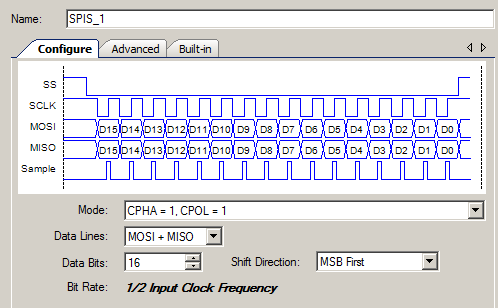
\includegraphics[scale=0.8]{tex/Design/SPI/Clock_mode_SPI}}
	\caption{Opsætning for SPI forbindelse Devkit8000-PSoC Master}
	\label{SPI_opsaetning}
\end{figure}

Ud fra figur \ref{SPI_opsaetning}, kan det aflæses at SPI clock mode er sat til CPHA = 1 og CPOL = 1, og antal databits sat til 16. Det PSoC program som var 
udleveret blev brugt som skabelon for gruppens eget program til PSoC master, dog med nogle modifikationer. Især håndteringen af de databits som blev modtaget 
fra devkittet blev genbrugt, da der ikke kunne ændres på disse bitkombinationer.

\myparagraph{PSoC Master - PSoC Slave}
\\
Til SPI forbindelsen mellem PSoC Master og PSoc slave havde gruppen frie hænder til opsætte SPI. Her blev clock mode valgt til CHPA = 0 og CPOL = 0, og 
antal databits til 8. Grunden til der kun bliver sendt 8 bits her, er at det er tilstrækkeligt til den simple form for kommunikation der er mellem PSoC-enhederne.
8 databits ville også have været fint for Devkit-PSoC forbindelsen, men som tidligere nævnt kunne det ikke ændres da der ikke var adgang til SPI device driveren
på Devkit8000. Clock mode er ændret til default værdien fra PSoC-Creator, efter inspektion af denne clock mode ligger der intet til grund for at den ikke
skulle virker fint. 
